\section{The Evolution of Chain-of-Thought}

\begin{frame}{}
    \LARGE Advanced Reasoning: \textbf{Chain-of-Thought Evolution}

    \vspace{1em}
    \normalsize One chain, many chains, a tree or a graph: what does each structure buy?
\end{frame}

\begin{frame}{The Family in One Picture}
    \centering
    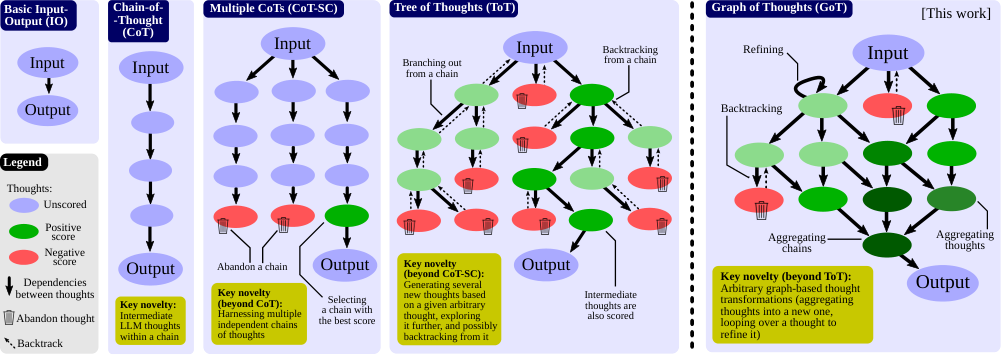
\includegraphics[width=\linewidth,height=0.54\textheight,keepaspectratio]{images/advanced-reasoning/got_fig1_topologies.png}
    \begin{itemize}\itemsep0.3em
        \item Read the family as shapes: a \textbf{path} (CoT), a \textbf{bundle} (Self-Consistency), a \textbf{planned sequence} (Least-to-Most), a \textbf{tree} (ToT), a \textbf{graph} (GoT).
        \item Each step adds one operation: vote, decompose, backtrack, aggregate. Each also needs something to \emph{score} thoughts.
    \end{itemize}
    \src{Besta et al., ``Graph of Thoughts: Solving Elaborate Problems with Large Language Models,'' AAAI 2024, \href{https://arxiv.org/abs/2308.09687}{arXiv:2308.09687}, Figure 1.}
\end{frame}

\begin{frame}{A Ladder of Selectors}
    \begin{itemize}\itemsep0.3em
        \item A vote counts answers. What if the output is free text, or the majority is wrong?
    \end{itemize}
    \begin{center}
    \small
    \renewcommand{\arraystretch}{1.2}
    \begin{adjustbox}{max width=\linewidth}\begin{tabular}{>{\raggedright\arraybackslash}p{3.3cm}>{\raggedright\arraybackslash}p{4.8cm}>{\raggedright\arraybackslash}p{5.6cm}}
        \toprule
        \textbf{Selector} & \textbf{How it chooses} & \textbf{Evidence} \\
        \midrule
        Self-Consistency & unweighted vote on the final answer & GSM8K with PaLM 2-L: greedy 85.7, vote 90.4 \\
        Universal Self-Consistency & the LLM reads all candidates and picks ``the most consistent'' & 90.2 on the same task. Also works on summaries and SQL, with no execution \\
        Verifier-weighted vote (DIVERSE) & a trained verifier weights each vote, step-aware & GSM8K 74.4 to 83.2 \\
        \rowcolor{KAUSTcyan!12} Exact verifier & tests, execution, a proof checker & the plateau disappears. Coverage becomes accuracy \\
        \bottomrule
    \end{tabular}\end{adjustbox}
    \end{center}
    \src{Chen et al., ``Universal Self-Consistency for LLM Generation,'' \href{https://arxiv.org/abs/2311.17311}{arXiv:2311.17311}, Table 1. Li et al., ``Making LLMs Better Reasoners with Step-Aware Verifier,'' \href{https://arxiv.org/abs/2206.02336}{arXiv:2206.02336}. Brown et al., \href{https://arxiv.org/abs/2407.21787}{arXiv:2407.21787}.}
\end{frame}

\begin{frame}{Least-to-Most: Chain-of-Thought with a Planner}
    \begin{columns}[T,onlytextwidth]
        \column{0.5\textwidth}
        \begin{itemize}\itemsep0.45em
            \item \textbf{Problem:} CoT fails on problems \emph{harder than its demonstrations}.
            \item \textbf{Method:} two prompted stages, no training. \emph{Decompose} into easier subproblems, then \emph{solve} them in order, each answer feeding the next.
            \item \textbf{SCAN, length split:} 99.7\% with 14 exemplars. CoT reaches 16.2\%.
            \item \textbf{The limit:} decomposition prompts transfer poorly across domains. Almost every failed GSM8K problem becomes solvable with a hand-written decomposition.
        \end{itemize}
        \column{0.47\textwidth}
        \centering
        \small
        \textbf{Last-letter concatenation, accuracy (\%)}

        \vspace{0.3em}
        \begin{adjustbox}{max width=\linewidth}\begin{tabular}{lccc}
            \toprule
            \textbf{List length} & \textbf{4} & \textbf{8} & \textbf{12} \\
            \midrule
            Standard prompt & 0.0 & 0.0 & 0.0 \\
            Chain-of-thought & 84.2 & 50.2 & 31.8 \\
            \rowcolor{KAUSTcyan!12} Least-to-Most & 94.0 & 83.0 & 74.0 \\
            \bottomrule
        \end{tabular}\end{adjustbox}

        \vspace{0.6em}
        \takeaway{Its value is \textbf{easy-to-hard generalisation}, not average accuracy. On GSM8K the gain appears only at 5 or more steps: 45.2 against 39.1.}
    \end{columns}
    \vspace{0.1em}
    \src{Zhou et al., ``Least-to-Most Prompting Enables Complex Reasoning in Large Language Models,'' ICLR 2023, \href{https://arxiv.org/abs/2205.10625}{arXiv:2205.10625}, Tables 4, 8 and 12. Model: code-davinci-002.}
\end{frame}

\begin{frame}{From Tree to Graph of Thoughts}
    \begin{itemize}\itemsep0.35em
        \item \textbf{Why a graph?} A tree can branch and backtrack, but it cannot \emph{merge} two good partial results.
        \item \textbf{Formalism.} Thoughts are vertices. Three transformations: \emph{generate} (as in ToT), \emph{aggregate} $k$ thoughts into one, \emph{refine} a thought in a loop.
    \end{itemize}
    \begin{center}
    \small
    \begin{adjustbox}{max width=\linewidth}\begin{tabular}{lcc}
        \toprule
        \textbf{Scheme, at total cost $\Theta(N)$} & \textbf{Latency} & \textbf{Volume of a thought} \\
        \midrule
        Chain-of-thought & $N$ & $N$ \\
        Self-Consistency, $k$ chains & $N/k$ & $N/k$ \\
        Tree-of-Thought, $k$-ary tree & $\log_k N$ & $O(\log_k N)$ \\
        \rowcolor{KAUSTcyan!12} Graph-of-Thought & $\log_k N$ & $N$ \\
        \bottomrule
    \end{tabular}\end{adjustbox}
    \end{center}
    \begin{itemize}\itemsep0.35em
        \item \emph{Volume}: how many earlier thoughts can influence a thought. Only the graph gets low latency \emph{and} high volume.
        \item Sorting 128 numbers with GPT-3.5: median error 62\% lower than ToT, at more than 31\% lower cost.
    \end{itemize}
    \src{Besta et al., \href{https://arxiv.org/abs/2308.09687}{arXiv:2308.09687}, Section 3 and Table 2.}
\end{frame}

\begin{frame}{When Does Chain-of-Thought Help at All?}
    \centering
    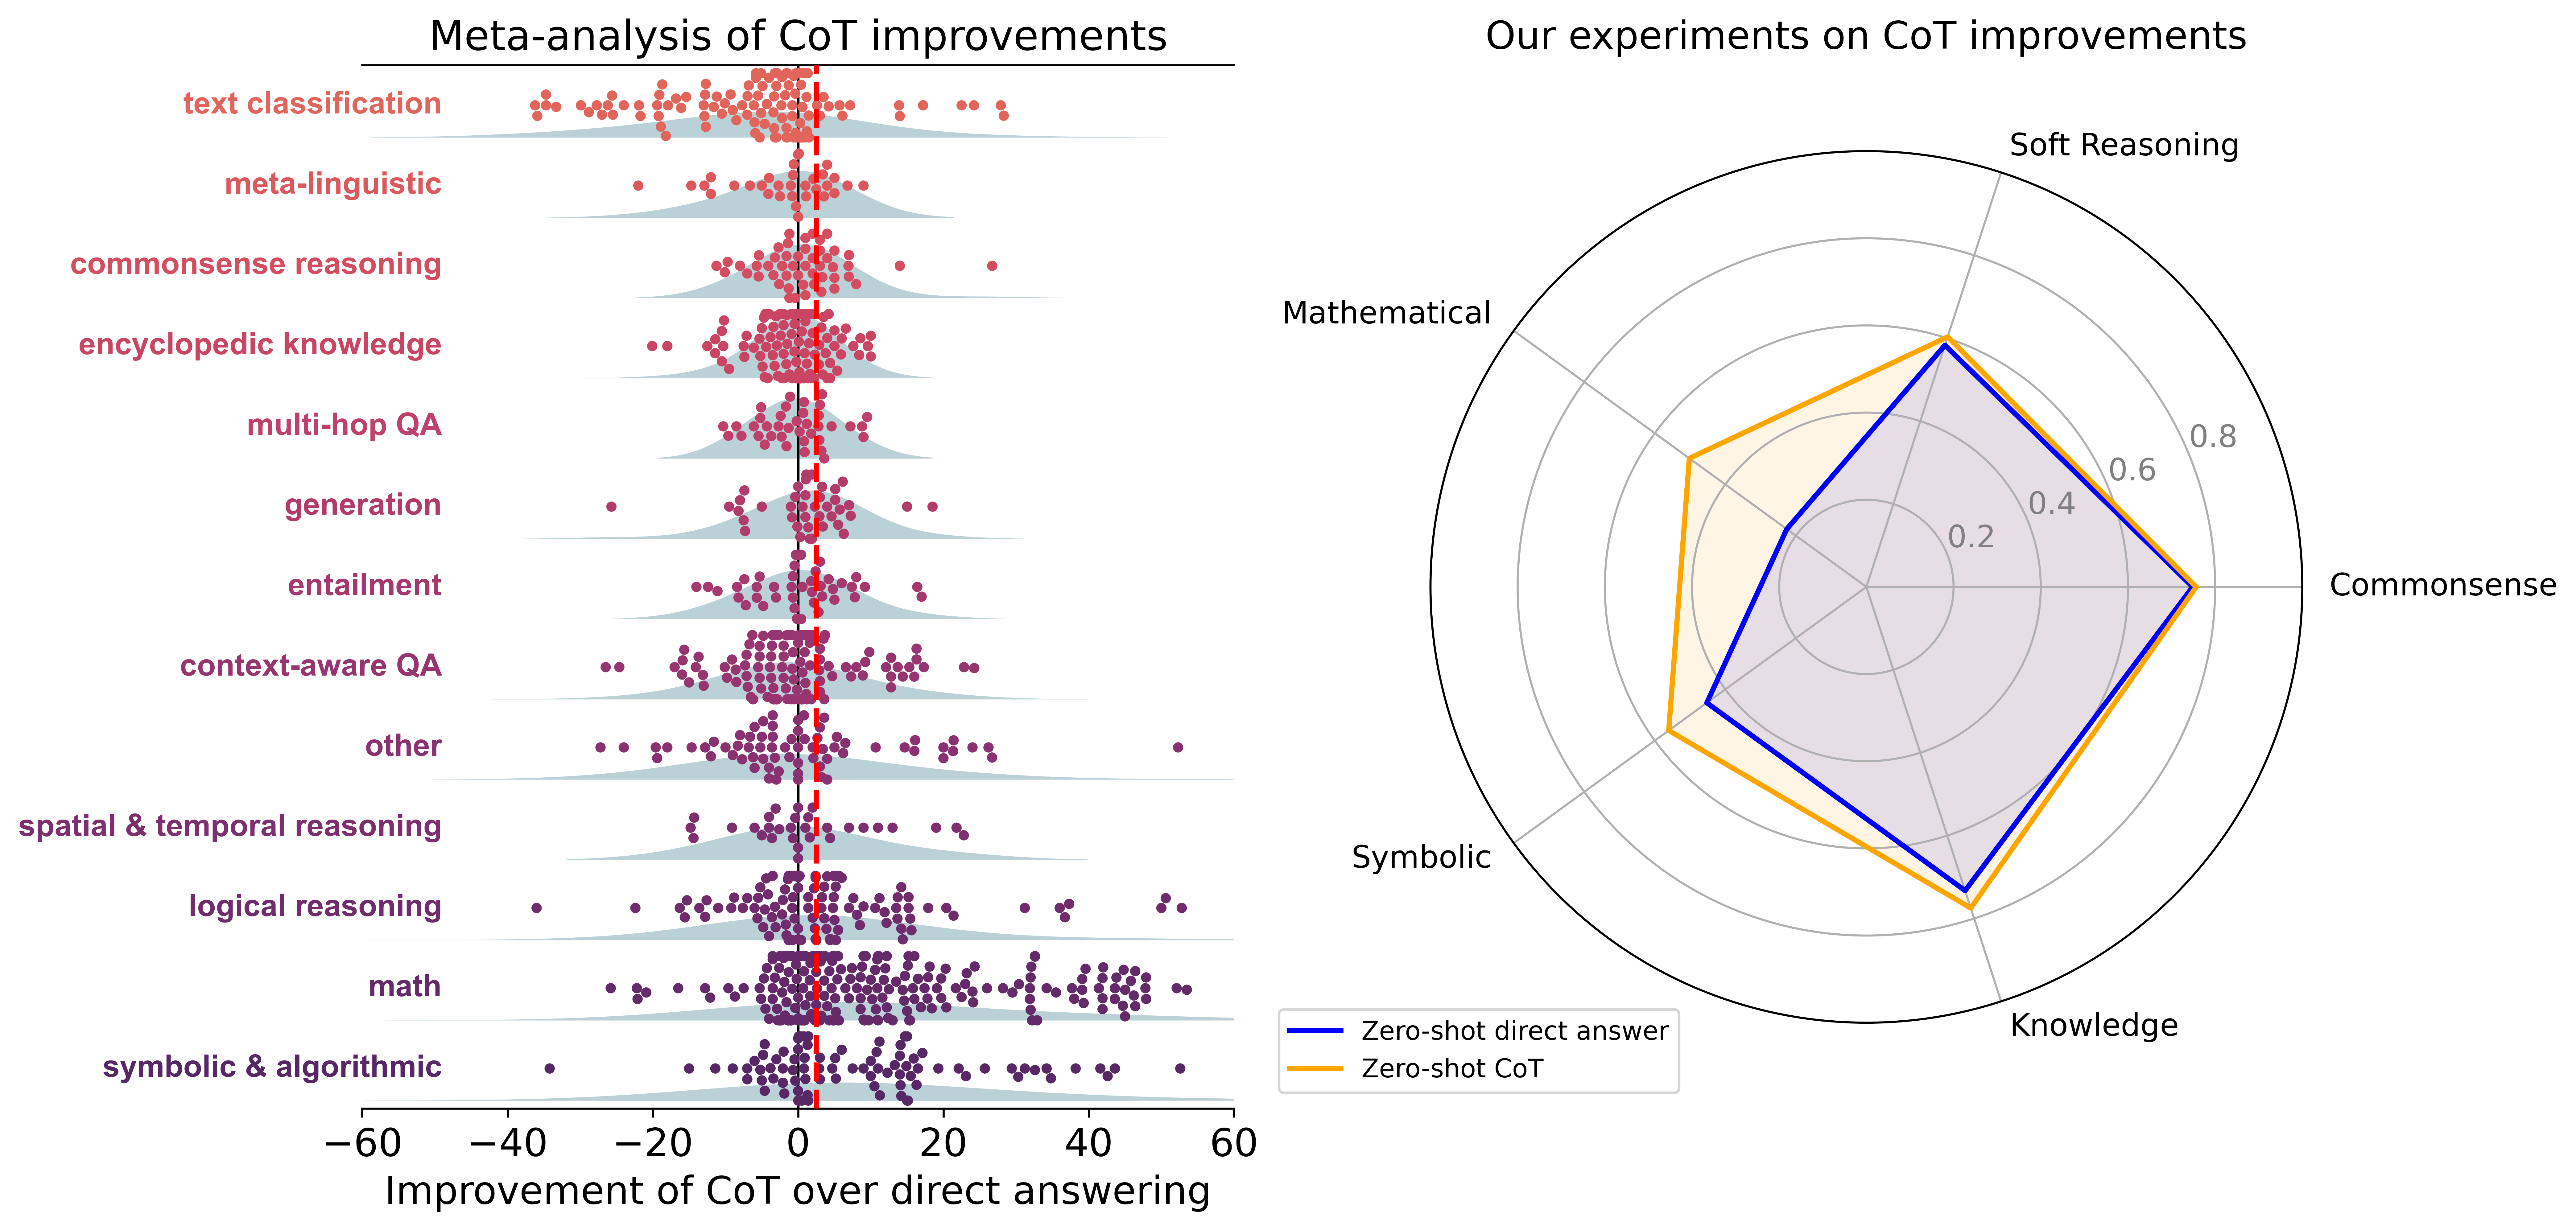
\includegraphics[width=0.9\linewidth,height=0.52\textheight,keepaspectratio]{images/advanced-reasoning/sprague_fig1_meta_analysis.png}
    \begin{itemize}\itemsep0.3em
        \item A meta-analysis of 1,218 comparisons from 110 papers, plus 20 datasets on 14 models.
        \item Average gain: \textbf{maths +12.3, symbolic +14.2, logic +6.9}. Everything else: +0.7.
        \item And where CoT helps, a planner plus a real \emph{tool} solver beats it. CoT is mostly symbolic execution, done badly.
    \end{itemize}
    \src{Sprague et al., ``To CoT or not to CoT?'' ICLR 2025, \href{https://arxiv.org/abs/2409.12183}{arXiv:2409.12183}, Figure 1. This studies \emph{prompted} CoT on 2024 models.}
\end{frame}

\begin{frame}{What Reasoning Models Made Obsolete}
    \begin{center}
    \small
    \renewcommand{\arraystretch}{1.05}
    \begin{adjustbox}{max width=\linewidth}\begin{tabular}{>{\raggedright\arraybackslash}p{3.4cm}>{\raggedright\arraybackslash}p{10.4cm}}
        \toprule
        \textbf{Status in 2026} & \textbf{Technique and evidence} \\
        \midrule
        \textbf{Superseded} & \emph{``Think step by step.''} On GPQA Diamond it changes o3-mini and o4-mini by about +0.03 and costs 20 to 80\% more time. On Gemini Flash 2.5 it hurts \\
        \textbf{Superseded} & \emph{Few-shot CoT exemplars.} ``Few-shot prompting consistently degrades'' R1. Five shots lowered o1-preview on MedQA \\
        \rowcolor{KAUSTcyan!12} \textbf{Still useful} & \emph{Voting and ensembling}, and explicit instructions on format and constraints \\
        \textbf{Moved inside the model} & \emph{Decomposition and search.} With thought and answer sampled together, ``the model can learn a search algorithm'' \\
        \bottomrule
    \end{tabular}\end{adjustbox}
    \end{center}
    \begin{itemize}\itemsep0.35em
        \item These structures were hand-designed. RL-trained models learn the structure inside one chain.
    \end{itemize}
    \src{Meincke et al., ``The Decreasing Value of Chain of Thought in Prompting,'' \href{https://arxiv.org/abs/2506.07142}{arXiv:2506.07142}. DeepSeek-AI, \href{https://arxiv.org/abs/2501.12948}{arXiv:2501.12948}. Nori et al., ``From Medprompt to o1,'' \href{https://arxiv.org/abs/2411.03590}{arXiv:2411.03590}. Welleck, CMU 11-711 (Nov 2025).}
\end{frame}

\begin{frame}{Chain-of-Thought Evolution: What to Remember}
    \begin{itemize}\itemsep0.6em
        \item The family is a sequence of shapes: \textbf{path, bundle, planned sequence, tree, graph}.
        \item Selectors climb a ladder: \textbf{vote, model pick, trained verifier, exact verifier}. Voting survives into the reasoning-model era. Prompted and few-shot CoT do not.
        \item Least-to-Most buys \textbf{length generalisation}. Graph-of-Thought buys \textbf{aggregation}.
        \item Prompted CoT helps mainly on \textbf{maths and symbolic} tasks, where a tool does better still.
    \end{itemize}
    \vspace{0.3em}
    \begin{block}{Zhou's four-line summary (2025)}
        Reasoning beats no reasoning. RL fine-tuning beats SFT. Aggregating several answers beats one answer. Retrieval plus reasoning beats reasoning alone.
    \end{block}
    \vspace{0.3em}
    \takeaway{\textbf{Next.} Trees and graphs need a rule for which thought to expand. That rule is \emph{search}, and it needs a scorer.}
\end{frame}
